\section{Experiments and evaluation}

In this section, we deploy our motion model from Equation~\eqref{eq:motionmodel} on our spherical mobile mapping system, shown in the left image of Figure~\ref{fig:calibstation}.
It is equipped with a ``Hesai PandarXT32'' LiDAR sensor and three ``Phidgets Spatial 3/3/3 1044b'' IMUs which are mounted rigidly inside the spherical shell of the system.
A ``BMAX B2ro'' Mini PC running Ubuntu Linux on an ``Intel Celeron N4120'' 4-core CPU ($\SI{2.6}{GHz}$) serves as the onboard processing unit. 
We currently roll the spherical system manually to record our datasets, yet we plan on including a locomotion mechanism, e.g., the ones mentioned in Section~\ref{sec:intro}, with future prototypes.
In this work, we compare the trochoidal motion model with two LIO methods: FAST-LIO~\cite{xu2022fast} and DLIO~\cite{10160508}, by utilizing an offline-batch continuous-time globally consistent SLAM algorithm, SRR~\cite{srr}, to provide reference trajectories.
\begin{figure*}
  \centering
  \includegraphics[width=.49\linewidth]{img/model3dtk}
  \includegraphics[width=.49\linewidth]{img/srr_trochoid}
  \caption{Left: The trajectory is the output of the trochoidal motion model, which is applied to the LiDAR data.
  Integration errors are present especially in the yaw axis leading to drift.
  Right: The LiDAR and trajectory data from the left image is used as input for SRR~\cite{srr}, which results in a globally consistent point cloud and trajectory.
  The color of the points denote intensity of the laser return.}
  \label{fig:srrtrochoid}
\end{figure*}
Figure~\ref{fig:srrtrochoid} shows that we use the output of the motion model directly as an initial guess for SRR, which outputs a globally consistent map and trajectory.
The latter serves as a reference to compare against the trajectories of the other three estimators.
Figure~\ref{fig:components} shows the position components for all 4 trajectories.
Qualitatively speaking, the motion model has notable drift in the yaw axis, which is due to the inability of the IMUs to provide reliable yaw estimations without the use of their magnetometer.
We forbid the use of the magnetometer by design because the prototype has been designed in an exoplanetary exploration context~\cite{deadalus}.
Notably, the motion model provides the most consistent estimate in the z-axis, where most of the trochoidal motion is happening.
Figure~\ref{fig:pointclouds} shows also the resulting point clouds when applying the trajectories to the LiDAR data in a zoomed sliced birds-eye view.
Again, the drift of the motion model, especially in the yaw axis, is apparent.
FAST-LIO has issues with scan matching leading to ghosting in the point cloud.
DLIO provides the best point cloud, although some residual error is still present, considering the misalignment of objects like chairs.

\subsection{Error metrics}

We have considered recording ground truth trajectory data with an external tracking system based on infrared markers, as we did in previous work~\cite{10256359}.
However, we have deliberately chosen not to do that in this paper due to tracking problems caused by marker reflections off the spherical shell and loss of vision on them when rolling.
To evaluate the accuracy of the estimated trajectories quantitatively, we compare them against the reference trajectory obtained by SRR.
We use the ``evo'' odometry evaluation tool from Grupp~\cite{grupp2017evo} to calculate the full absolute pose error (APE) of the trajectories, which splits into two parts: position and rotation error.
\begin{itemize}
  \item \textbf{Position error:}\\
  The absolute pose error with respect to position in meters ($\mathrm{APE\;[m]}$) represents the unsigned error for each pose between the estimated position $\vec{p}_{\mathrm{est},i}$ and refernce position $\vec{p}_{\mathrm{ref},i}$
  \begin{equation}
      \lvert \vec{p}_{\mathrm{est},i} - \vec{p}_{\mathrm{ref},i} \rvert \;.
      \label{eq:ape}
  \end{equation}

  \item \textbf{Rotation error:}\\
  The abolute pose error with respect to rotation in degrees ($\mathrm{APE\;[\phantom{.}^{\circ}]}$) represents the error for each pose between the orientation estimation $\vec{R}_{\mathrm{est},i}$ and the orientation reference $\vec{R}_{\mathrm{est},i}$
  \begin{equation}
      \left| \angle \left( \vec{R}_{\mathrm{est},i}^{-1} \vec{R}_{\mathrm{ref},i} \right)\right| \;.
      \label{eq:rpe}
  \end{equation}
\end{itemize}

\subsection{Results}
Metrics for both individual components of the APE are listed in Table~\ref{tab:apetable}, whereas the full APE for each trajectory is plotted in Figure~\ref{fig:ape}.
The results indicate that the motion model is outperformed by DLIO and FAST-LIO, especially for the rotation part, which is unsurprising since these methods use additional LiDAR data instead of only magnetometer-denied IMU data.
However, the metrics are in the same order of magnitude and the motion model seems to perform better than FAST-LIO regarding the positional error for some metrics.
We make that statement cautiously, though, since the motion model alone has no way of recovering from the accumulated drift in longer trajectories.
It is for this reason, that we plan to implement the motion model into a LIO method specifically tailored towards spherical systems.
Our results show that both FAST-LIO and DLIO do perform sub-optimally in this context, and also that our motion model has the potential to aid such methods to reach their full capabilities which have been demonstrated in their respective papers~\cite{xu2022fast, 10160508}. 
Furthermore, keep in mind that the LIO methods only provide their pose estimates at the LiDAR frequency, $\SI{20}{Hz}$ in our case, whereas the motion model provides them at the higher IMU frequency which is $\SI{125}{Hz}$.

\begin{figure}
  \centering 
  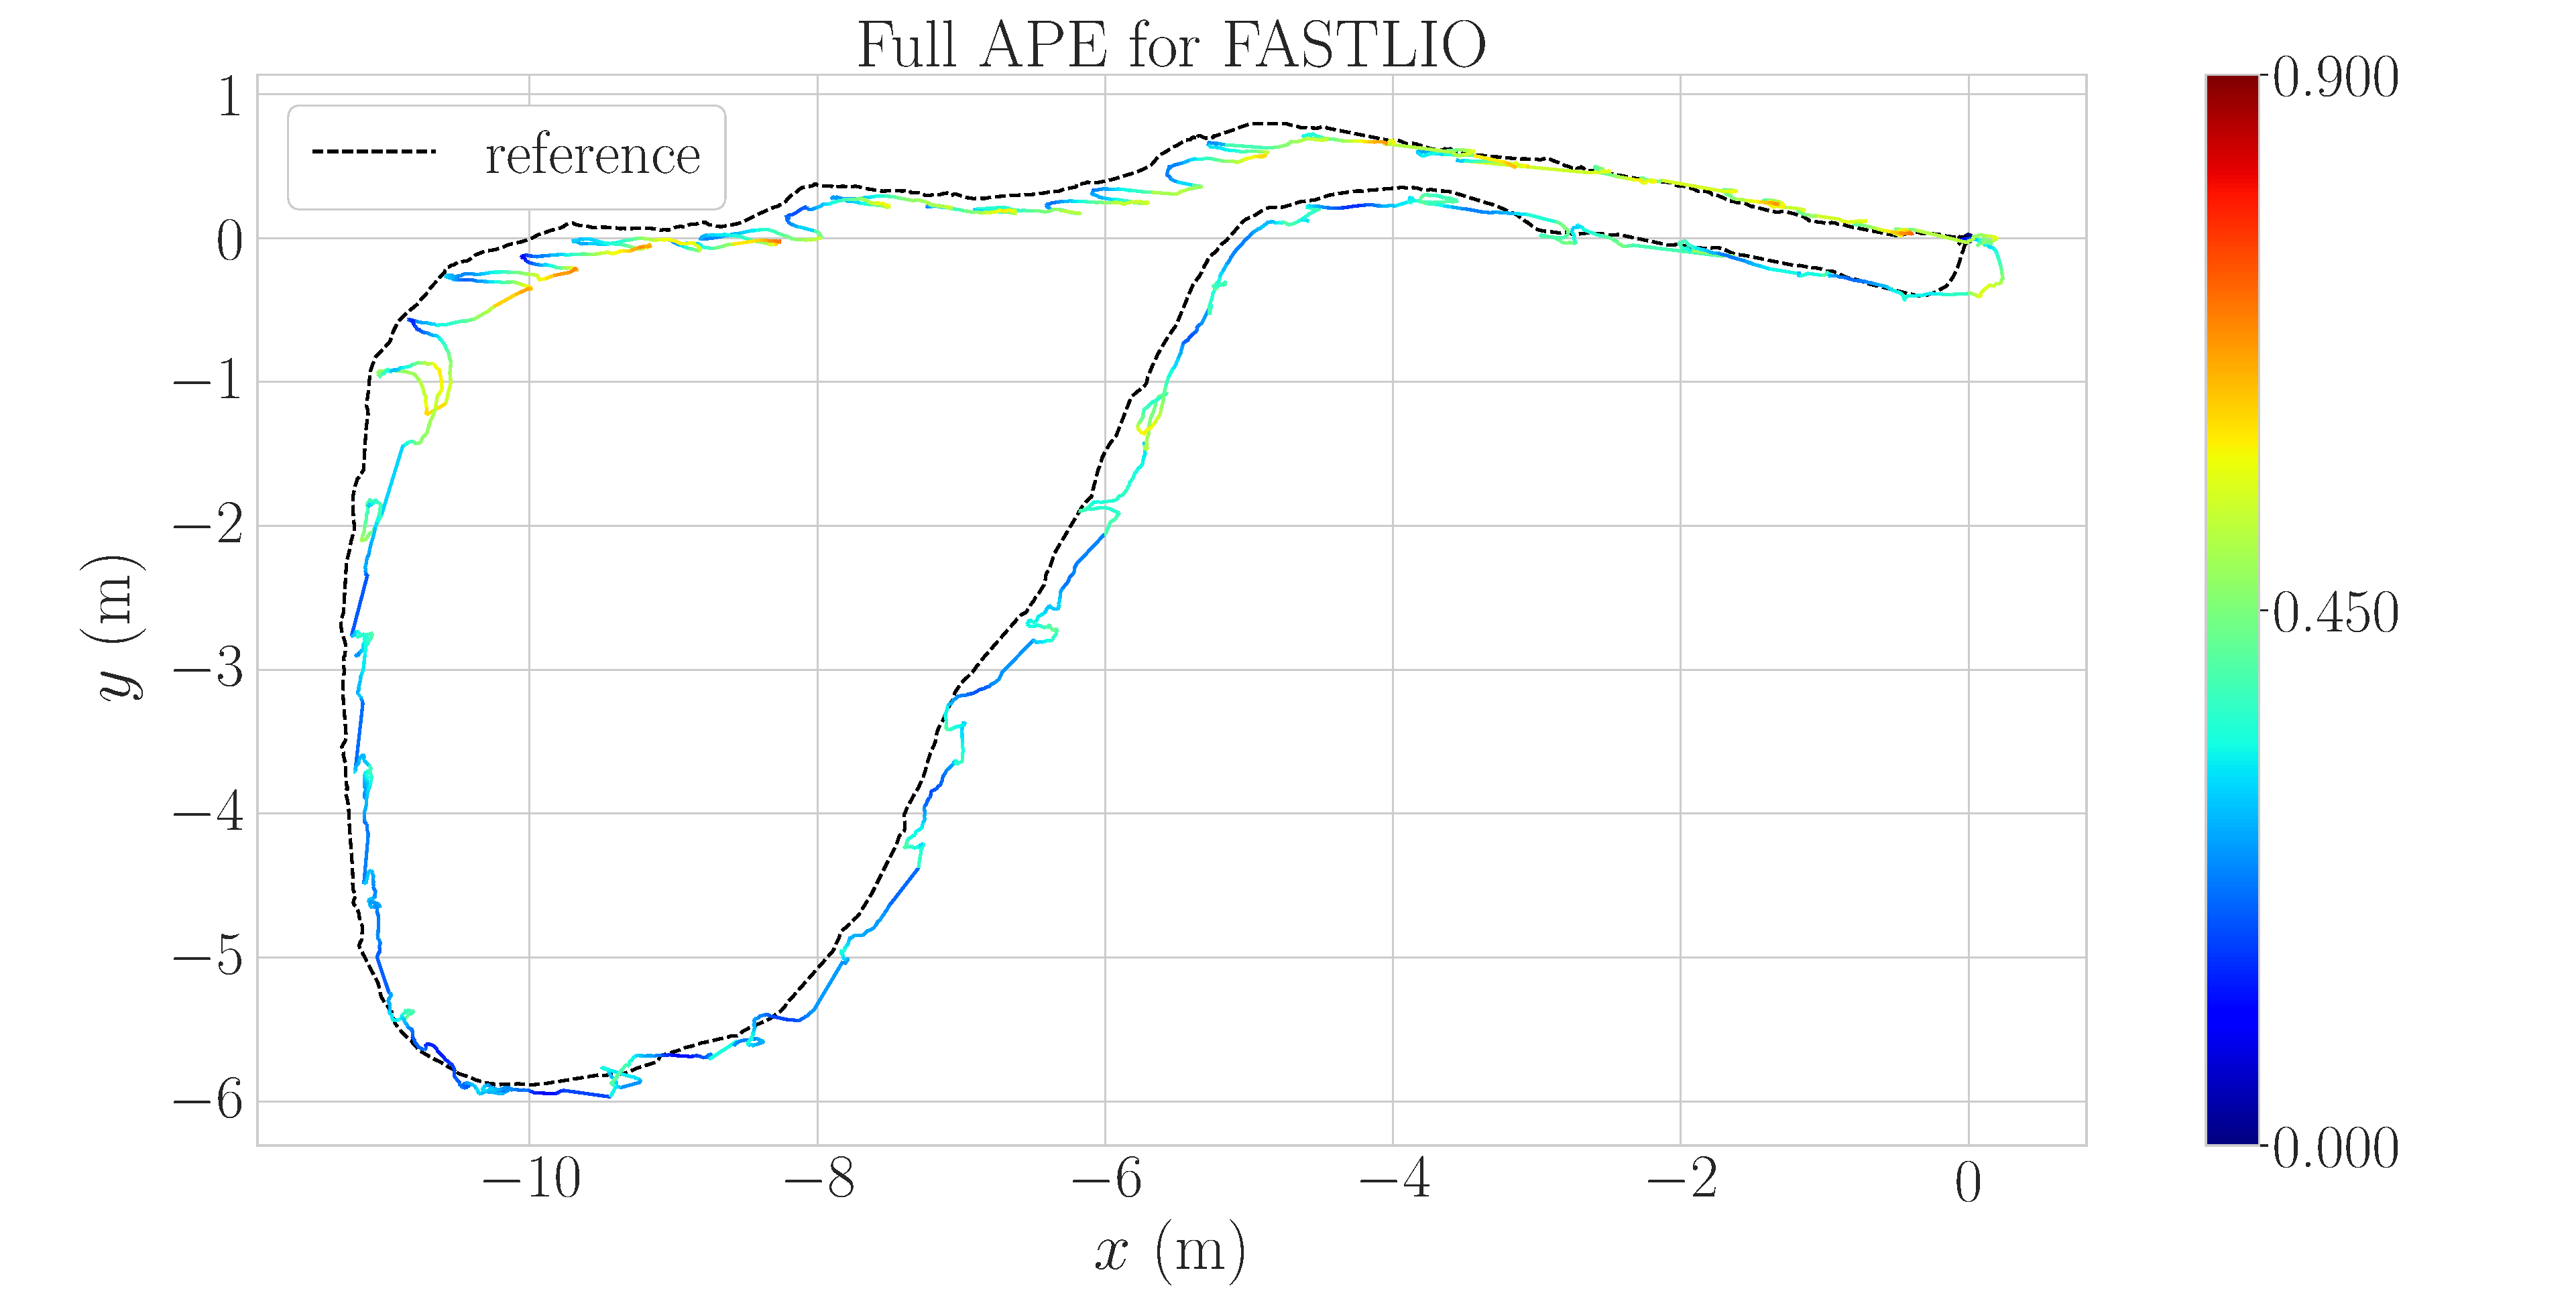
\includegraphics[width=\linewidth]{img/ape_fast_lio} \vskip 2mm
  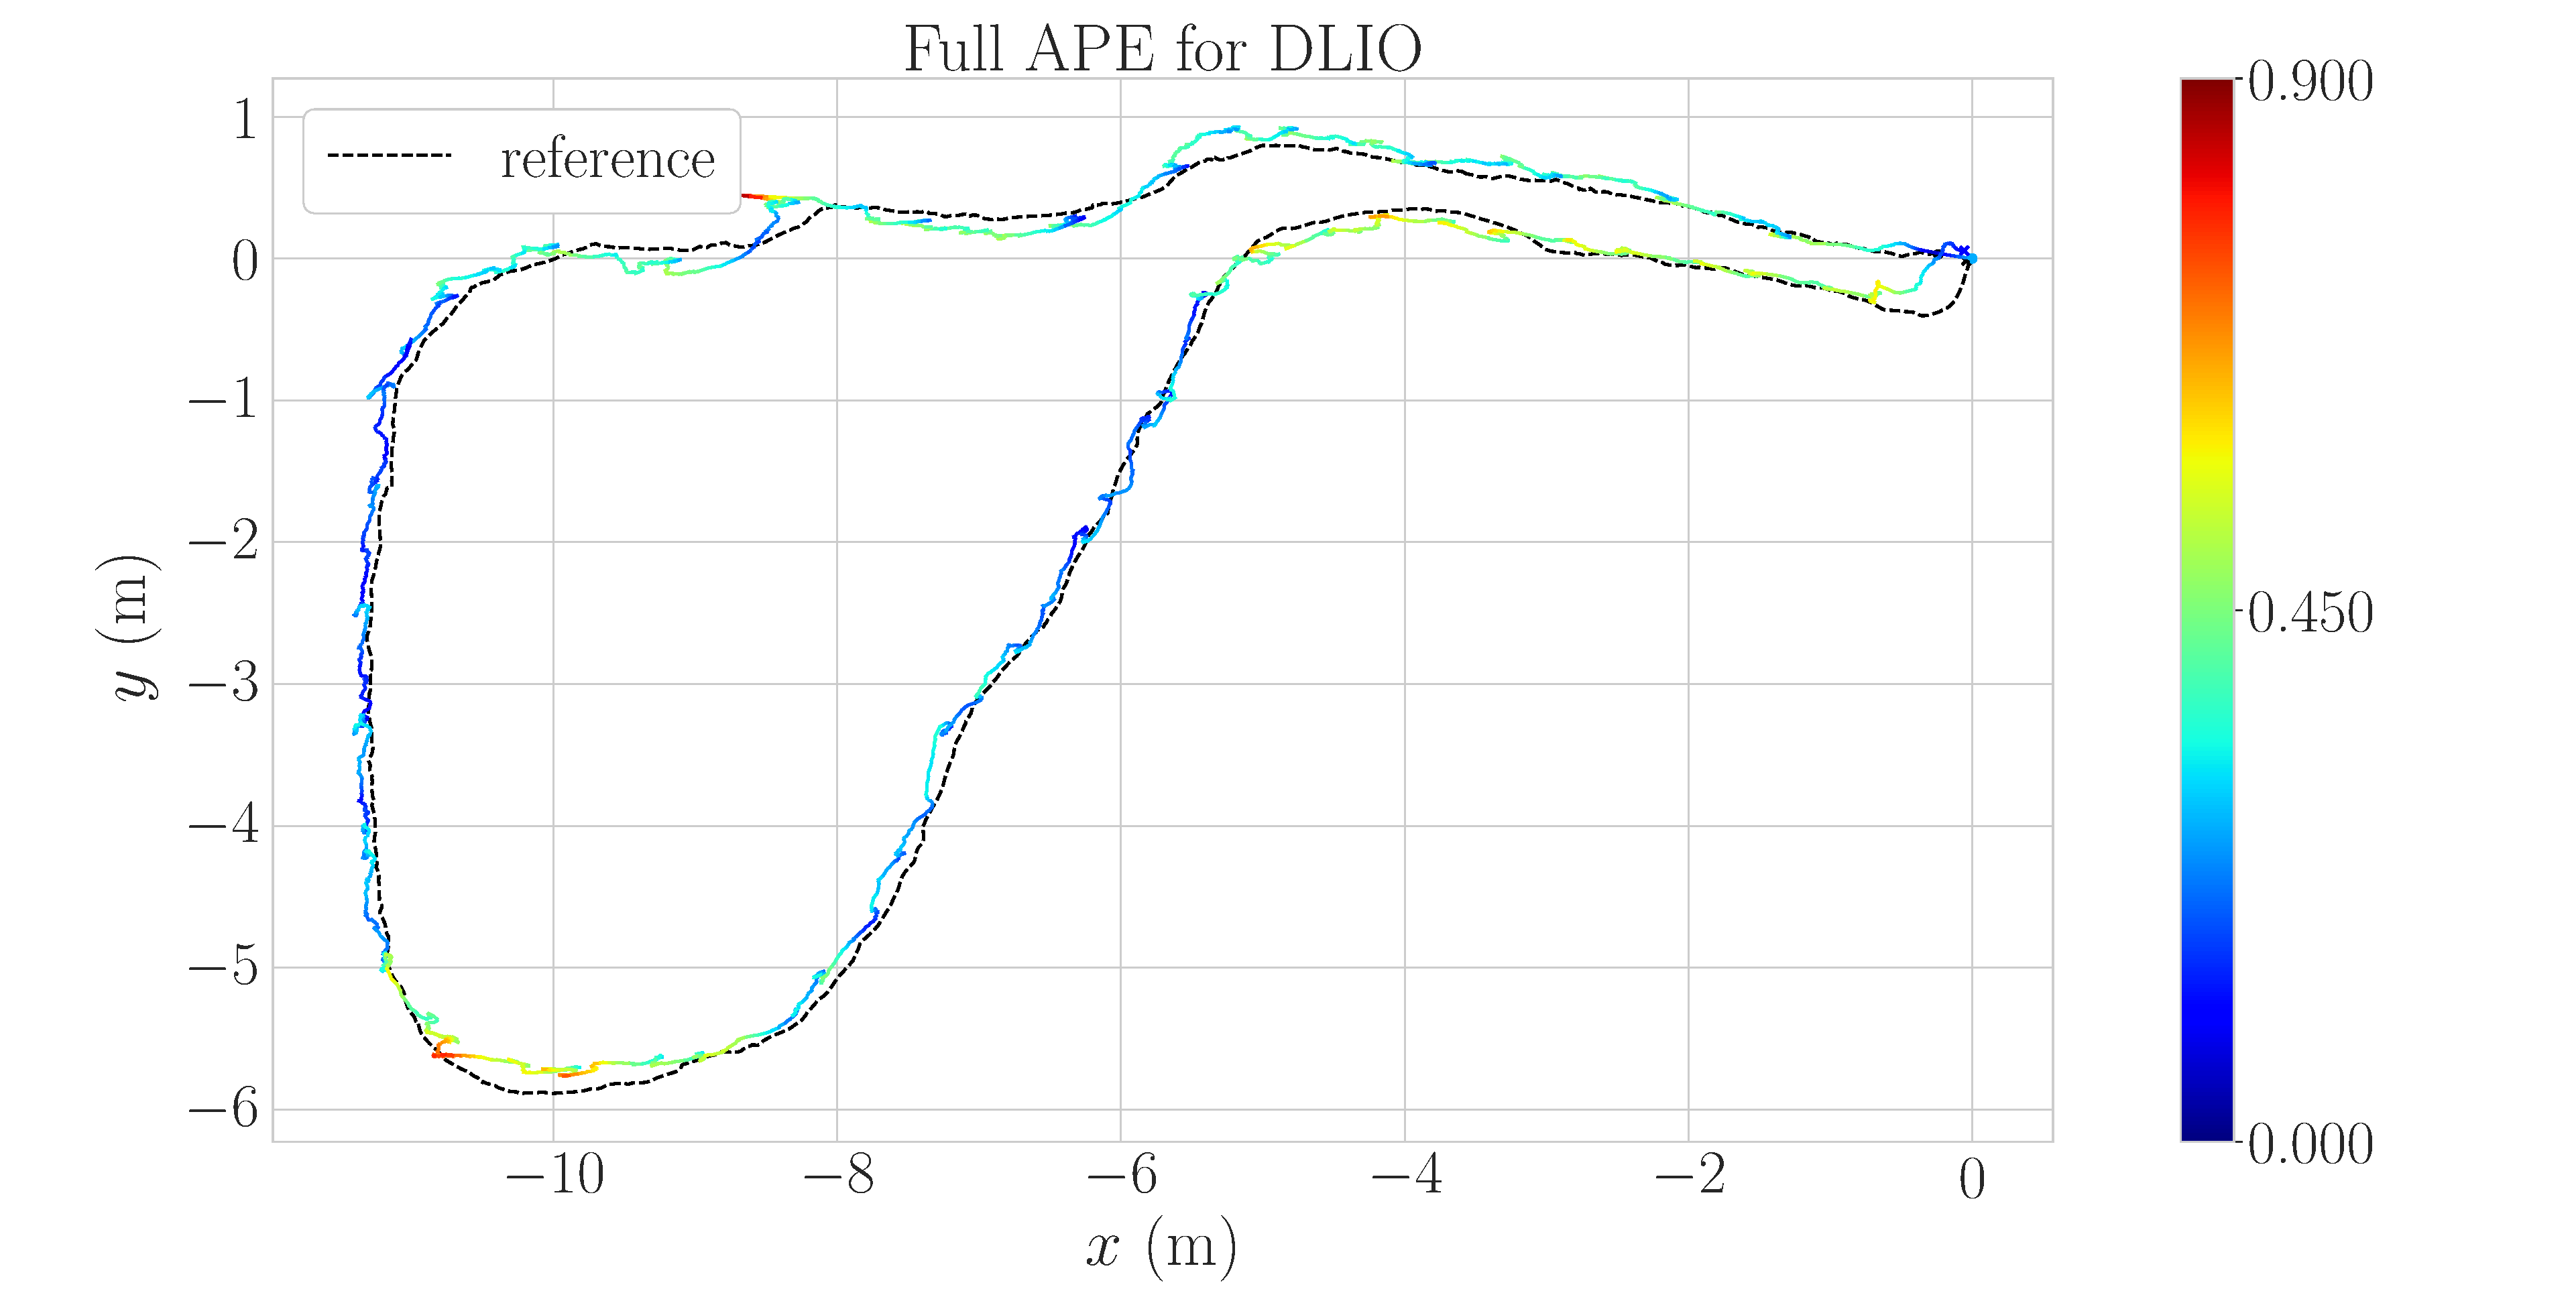
\includegraphics[width=\linewidth]{img/ape_dlio} \vskip 2mm
  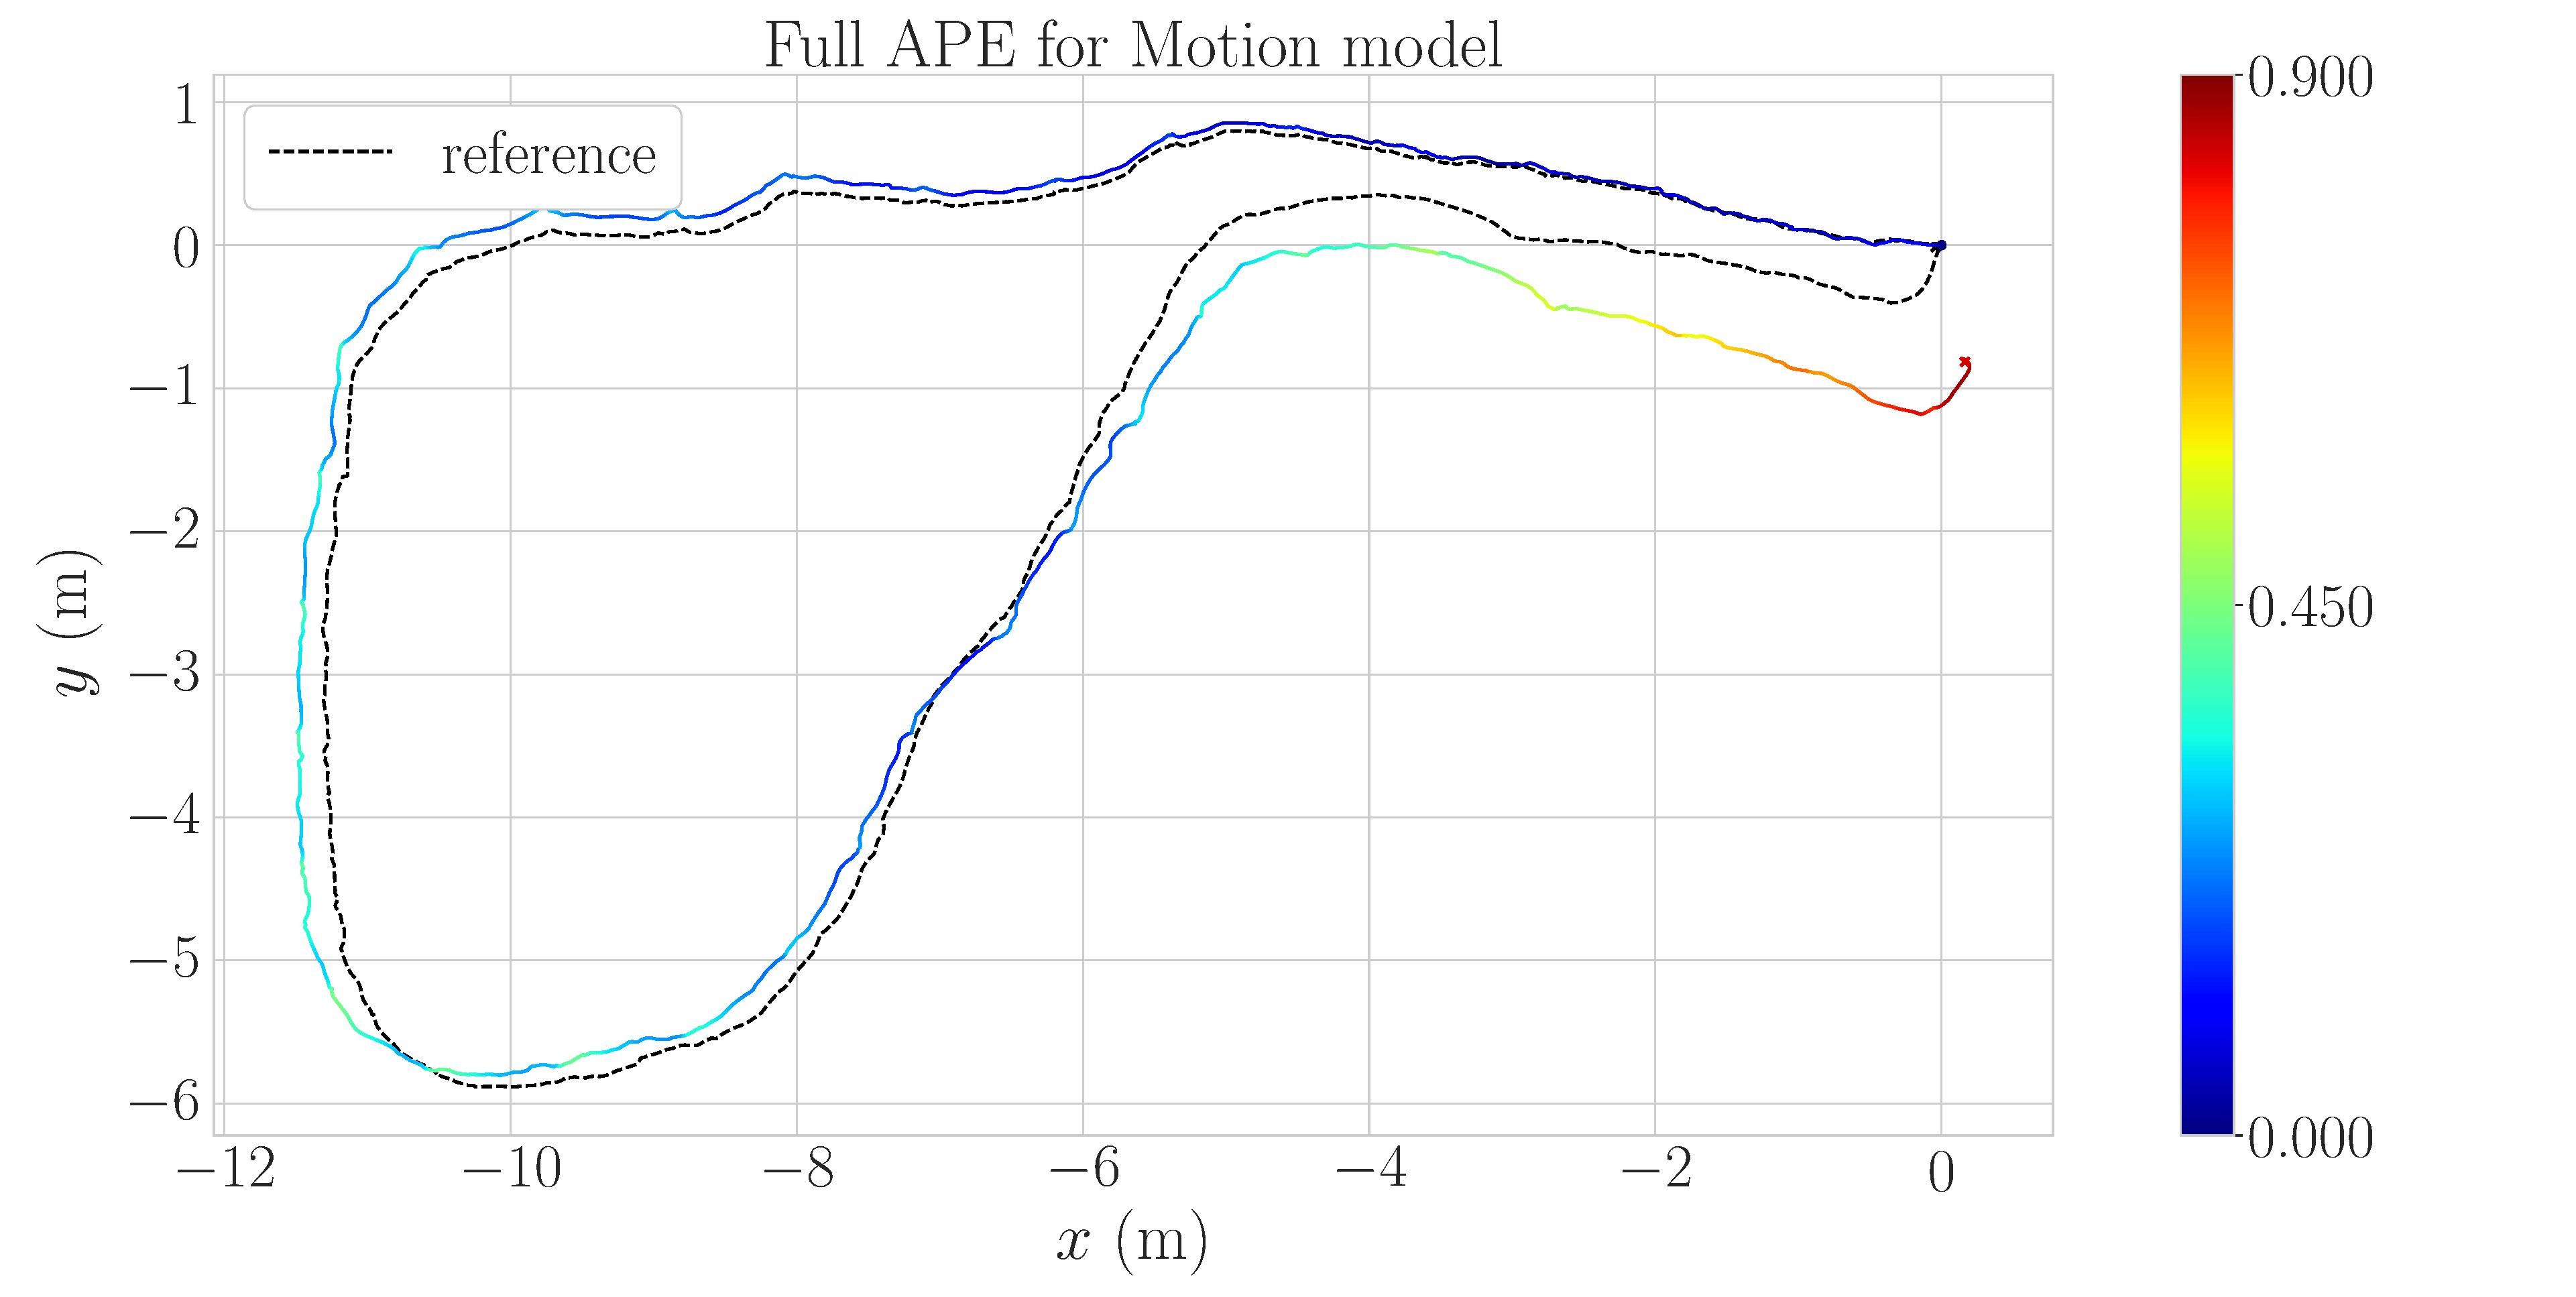
\includegraphics[width=\linewidth]{img/ape_model}
  \caption{Comparison of the estimated trajectories.
  The color denotes the combined absolute pose error (unit-less).
  Our motion model experiences drift, the LIO methods inconsistently jump.}
  \label{fig:ape}
\end{figure}

\begin{figure}
  \centering 
  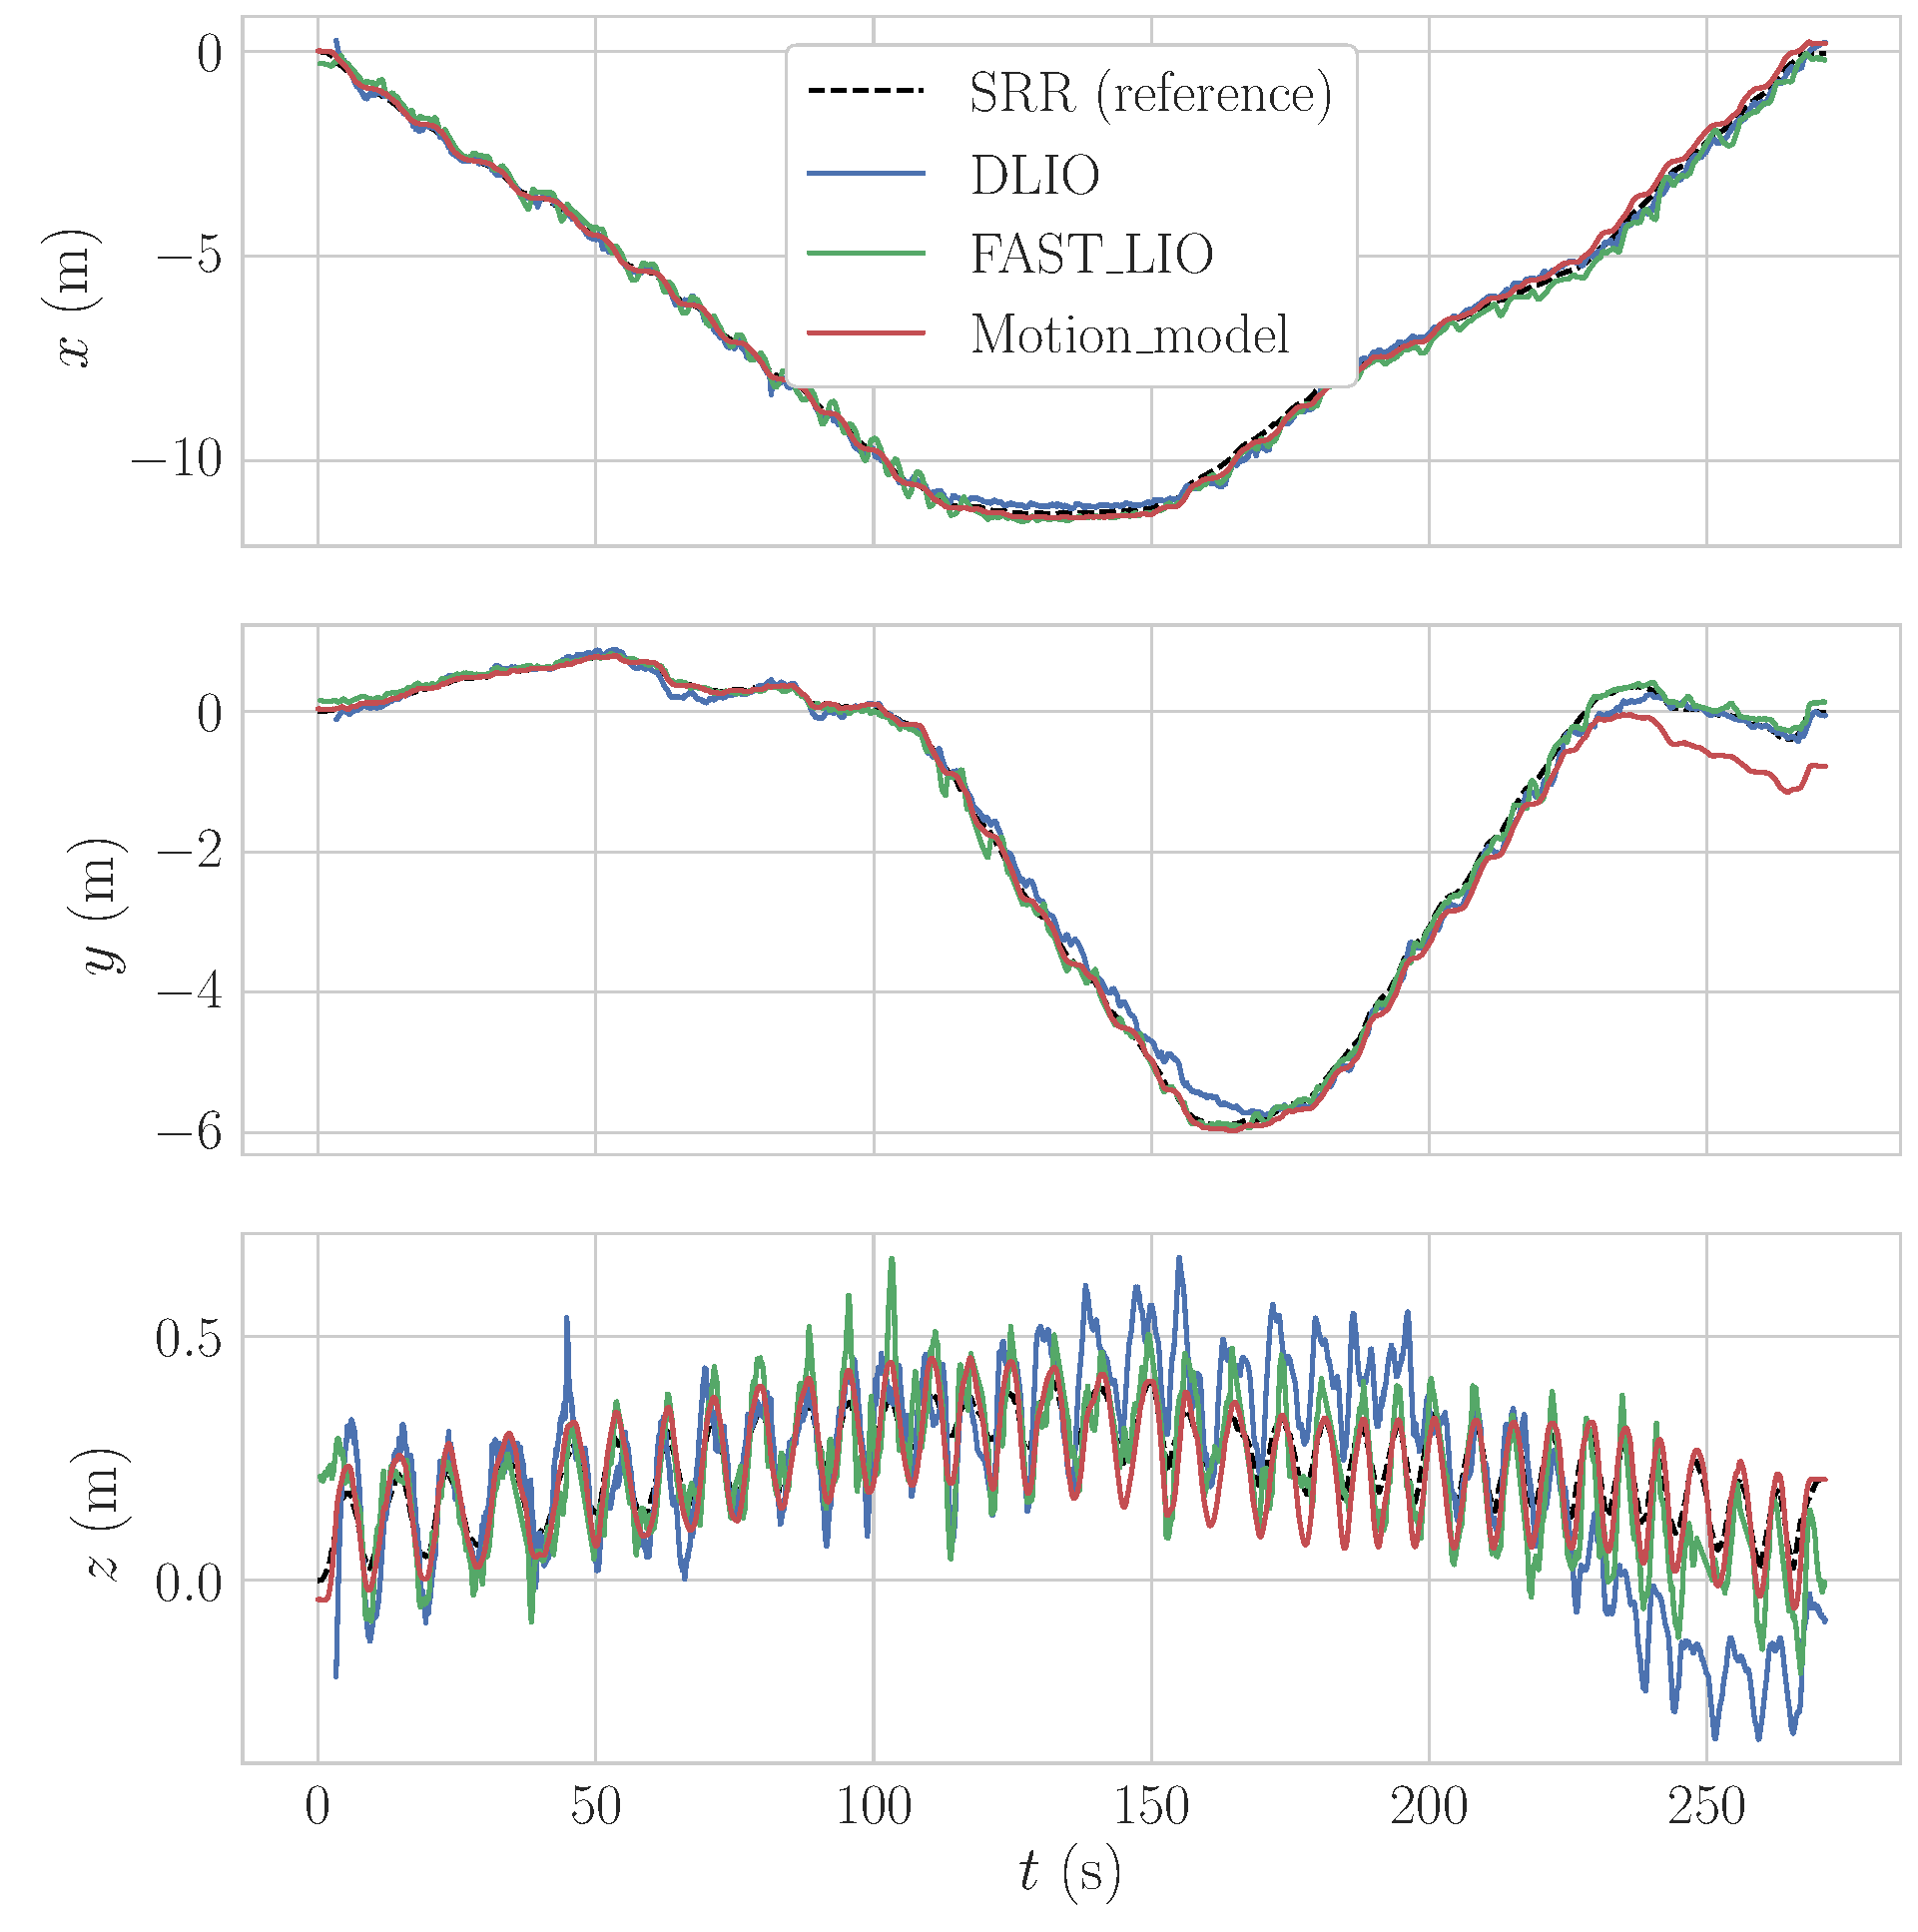
\includegraphics[width=\linewidth]{img/trajectory_components}
  \caption{Component-wise comparison of the estimated trajectories.
  The trochoidal nature of the LiDAR trajectory is best represented by the motion model.}
  \label{fig:components}
\end{figure}

\begin{figure*}
  \centering 
  \subfloat[Motion model + SRR (reference) \label{fig:srr_detail}]{%
    \includegraphics[width=.49\linewidth]{img/srr_detail}}%
  \subfloat[Motion model (IMU only) \label{fig:model_detail}]{%
    \includegraphics[width=.49\linewidth]{img/model_detail}}%
  \hfill \vskip 2mm 
  \subfloat[FAST\_LIO \label{fig:fastlio_detail}]{%
    \includegraphics[width=.49\linewidth]{img/fastlio_detail}}%
  \subfloat[DLIO \label{fig:dlio_detail}]{%
    \includegraphics[width=.49\linewidth]{img/dlio_detail}}%
  \hfill
  \caption{Comparison of the estimated trajectories and resulting point clouds in a zoomed, sliced birds-eye view.
  The color of the points denote the intensity of the LiDAR return signal.
  Only in the reference point cloud every object is aligned.
  The motion model drifts, FAST-LIO has ghosting, and DLIO has misaligned objects.}
  \label{fig:pointclouds}
\end{figure*}

\begin{table*}
  \centering 
  \vskip 3mm
  \caption{Comparison of statistical metrics for the positional and rotational components of the absolute pose error (APE) for all compared estimators.
  The best value is printed in \textbf{bold}, the second best in \textit{italics} numbers where lower is better.}
  \label{tab:apetable}
  \resizebox{\textwidth}{!}{%
  \begin{tabular}{|p{2.5cm}||p{1.0cm}|p{1.0cm}|p{1.0cm}|p{1.0cm}|p{1.0cm}|p{1.0cm}|p{1.0cm}|p{1.0cm}|p{1.0cm}|p{1.0cm}|}
    \hline
    \multirow{2}{*}{Estimator} &
      \multicolumn{2}{c}{Median} &
      \multicolumn{2}{c}{Mean} &
      \multicolumn{2}{c}{Std.} &
      \multicolumn{2}{c}{RMSE} &
      \multicolumn{2}{c|}{Max.}\\
    & APE~[m] & APE~[$\phantom{l}^{\circ}$] & APE~[m] & APE~[$\phantom{l}^{\circ}$] & APE~[m] & APE~[$\phantom{l}^{\circ}$] & APE~[m] & APE~[$\phantom{l}^{\circ}$] & APE~[m] & APE~[$\phantom{l}^{\circ}$]\\
    \hline
    DLIO & \textbf{0.230} & \textbf{4.345} & \textbf{0.230} & \textit{4.456} & \textbf{0.085} & \textit{1.791} & \textbf{0.245} & \textit{4.637} & \textbf{0.579} & 10.675\\
    \hline
    FASTLIO & 0.413 & \textit{4.356} & 0.428 & \textbf{4.436} & \textit{0.116} & \textbf{1.247} & 0.444 & \textbf{4.487} & \textit{0.758} & \textbf{8.922}\\
    \hline
    Motion model & \textit{0.246} & 4.748 & \textit{0.272} & 4.457 & 0.179 & 1.940 & \textit{0.326} & 4.861 & 0.877 & \textit{8.968}\\
    \hline
  \end{tabular}}
\end{table*}

